% ============================================================
% Rapport de Stage de Fin d'Études
% Soumaya Amallal — EST Ouarzazate 2025/2026
% ============================================================
\documentclass[12pt,a4paper]{report}

% ── Encodage & langue ────────────────────────────────────────

\usepackage[utf8]{inputenc}
\usepackage[T1]{fontenc}
\usepackage[nil]{babel}

% ── Mise en page ─────────────────────────────────────────────
\usepackage[top=2.5cm,bottom=2.5cm,left=3cm,right=2.5cm]{geometry}
\usepackage{setspace}
\onehalfspacing

% ── Polices & couleurs ───────────────────────────────────────

\usepackage{xcolor}
\definecolor{darkblue}{HTML}{1a2744}
\definecolor{midblue}{HTML}{2e4a8a}
\definecolor{accentred}{HTML}{c0392b}
\definecolor{lightgray}{HTML}{f2f4f7}
\definecolor{graytext}{HTML}{444444}

% ── Titres personnalisés ─────────────────────────────────────
\usepackage{titlesec}
\titleformat{\chapter}[display]
  {\normalfont\huge\bfseries\color{darkblue}}
  {\chaptertitlename\ \thechapter}{20pt}{\Huge}
\titlespacing*{\chapter}{0pt}{-30pt}{20pt}
\titleformat{\section}
  {\normalfont\Large\bfseries\color{midblue}}
  {\thesection}{1em}{}
\titleformat{\subsection}
  {\normalfont\large\bfseries\color{darkblue}}
  {\thesubsection}{1em}{}
\titleformat{\subsubsection}
  {\normalfont\normalsize\bfseries\color{graytext}}
  {\thesubsubsection}{1em}{}

% ── Tableaux ─────────────────────────────────────────────────
\usepackage{booktabs}
\usepackage{array}
\usepackage{tabularx}
\usepackage{longtable}
\usepackage{multirow}
\usepackage[table]{xcolor}
\newcolumntype{L}[1]{>{\raggedright\arraybackslash}p{#1}}
\newcolumntype{C}[1]{>{\centering\arraybackslash}p{#1}}

% ── Graphiques & figures ─────────────────────────────────────
\usepackage{graphicx}
\usepackage{float}
\usepackage{caption}
\captionsetup{font=small,labelfont=bf,textfont=it}

% ── Mathématiques ────────────────────────────────────────────
\usepackage{amsmath}
\usepackage{amssymb}

% ── Boîtes & encadrés ───────────────────────────────────────
\usepackage{tcolorbox}
\tcbuselibrary{skins,breakable}

\newtcolorbox{infobox}{
  enhanced, breakable,
  colback=lightgray,
  colframe=midblue!40,
  boxrule=0.5pt,
  left=8pt, right=8pt, top=6pt, bottom=6pt,
  fontupper=\small\itshape
}

\newtcolorbox{statusbox}{
  enhanced, breakable,
  colback=blue!5,
  colframe=midblue,
  boxrule=0.8pt,
  left=8pt, right=8pt, top=6pt, bottom=6pt,
  fontupper=\small
}

% ── En-têtes & pieds de page ─────────────────────────────────
\usepackage{fancyhdr}
\pagestyle{fancy}
\fancyhf{}
\fancyhead[L]{\small\textcolor{graytext}{Rapport de Stage Technique --- EST Ouarzazate 2025/2026}}
\fancyhead[R]{}
\fancyfoot[C]{\thepage}
\renewcommand{\headrulewidth}{0.4pt}

% ── Hyperliens ───────────────────────────────────────────────
\usepackage[hidelinks,colorlinks=false]{hyperref}

% ── Listes ──────────────────────────────────────────────────
\usepackage{enumitem}
\setlist[itemize]{leftmargin=1.5em, topsep=4pt, itemsep=2pt}

% ── Numérotation des figures/tableaux par chapitre ───────────
\usepackage{chngcntr}
\counterwithin{figure}{chapter}
\counterwithin{table}{chapter}

% ── Divers ──────────────────────────────────────────────────
\usepackage{lipsum}
\usepackage{needspace}


% ============================================================
\begin{document}

% ── PAGE DE TITRE ────────────────────────────────────────────
\begin{titlepage}
\centering

% ── Logos en haut ────────────────────────────────────────────
\noindent
\begin{minipage}[c]{0.38\textwidth}
  \centering
  \includegraphics[width=3.5cm]{images/ormvao.png}
\end{minipage}
\hfill
\begin{minipage}[c]{0.58\textwidth}
  \centering
  
\includegraphics[width=7cm]{images/est_logo.png}
\end{minipage}

\vspace*{2cm}

\begin{center}

{\Huge\bfseries\color{darkblue}
Rapport de Stage Technique
}

\vspace{1.8cm}

\begin{tcolorbox}[
    enhanced,
    colback=white,
    colframe=white,
    width=0.92\textwidth,
    boxrule=0pt
]

\centering

{\Huge\bfseries
Cartographie et Analyse
}

\vspace{0.4cm}

{\Huge\bfseries
du Risque Potentiel d'Incendie
}

\vspace{0.4cm}

{\LARGE\bfseries
dans la Région d'Agdz
}

\vspace{1.2cm}

\noindent
\color{darkblue}
\rule{0.75\textwidth}{1.2pt}

\vspace{0.8cm}

{\large\itshape
À l'aide de la Télédétection, des Données Climatiques\\[0.3cm]
et de l'Intelligence Artificielle
}

\vspace{0.2cm}

\color{darkblue}
\rule{0.75\textwidth}{1.2pt}

\end{tcolorbox}

\end{center}
\vspace{1.5cm}
\begin{tabular}{rl}
\textbf{Réalisé par :}            & Soumaya Amallal \\[4pt]
\textbf{Encadrante pédagogique :} & Mme. Wassima Aït Farès \\[4pt]
\textbf{Entreprise d'accueil :}   & ORMVAO --- Ouarzazate \\[4pt]
\textbf{Encadrant professionnel :}& M. El Achaoui Youssef \\[4pt]
\textbf{Période de stage :}       & Du 06 avril 2026 au 06 juin 2026 \\[4pt]
\textbf{Année universitaire :}    & 2025 / 2026 \\
\end{tabular}

\end{titlepage}  % <-- CORRECTION : \end{titlepage} manquant dans l'original


% ── DÉDICACE ─────────────────────────────────────────────────
\chapter*{Dédicace}
\addcontentsline{toc}{chapter}{Dédicace}
\thispagestyle{empty}

\begin{center}
\itshape
À mes très chers parents,\\
dont l'amour inconditionnel, les sacrifices silencieux\\
et la confiance indéfectible ont été le socle\\
de chacune de mes réussites.\\
Aucun mot ne saurait exprimer ma gratitude profonde.\\[1em]

À mes sœurs bien-aimées,\\
complices de toujours, sources de joie et de sérénité,\\
pour leur soutien fraternel et leur présence lumineuse.\\[1em]

À toute ma famille,\\
pour l'élan de bienveillance et d'encouragement\\
qui m'a portée tout au long de ce parcours.\\[1em]

À mes amis et camarades de promotion,\\
pour les moments de partage, d'entraide\\
et de solidarité qui ont enrichi ces années d'études.\\[1em]

À mes professeurs et enseignants,\\
qui m'ont transmis le savoir, la rigueur\\
et la passion pour la donnée et la science.\\[1em]

Je dédie ce travail à chacun d'entre vous,\\
avec tout mon respect et toute mon affection.
\end{center}

% ── REMERCIEMENTS ────────────────────────────────────────────
\chapter*{Remerciements}
\addcontentsline{toc}{chapter}{Remerciements}

Ce travail n'aurait pu voir le jour sans la contribution précieuse de nombreuses personnes. Qu'il me soit permis de leur exprimer ici ma plus sincère et profonde reconnaissance.

Je tiens, en premier lieu, à adresser mes remerciements les plus respectueux et les plus chaleureux à \textbf{Monsieur Ahmed El Bouari}, Directeur Adjoint de l'ORMVAO, pour l'accueil bienveillant qu'il m'a réservé au sein de son établissement et pour les conditions de travail exemplaires qu'il a su mettre en place.

J'exprime ma gratitude la plus sincère à \textbf{Monsieur El Achaoui Youssef}, Chef du Bureau des Formations et encadrant professionnel de ce stage, pour son accompagnement rigoureux et constant tout au long de cette période. Ses précieux conseils et sa grande compétence ont été des atouts majeurs dans la conduite de ce projet.

Mes remerciements les plus profonds vont à \textbf{Madame Wassima Aït Farès}, encadrante pédagogique à l'EST Ouarzazate, pour son suivi assidu, ses remarques constructives et la qualité de son encadrement. Ses orientations académiques ont été déterminantes dans la structuration scientifique de ce travail.

Je remercie également l'ensemble du corps enseignant de l'EST Ouarzazate et les responsables de la filière Ingénierie des Données pour la formation solide et pluridisciplinaire qu'ils m'ont dispensée.

Je tiens à exprimer ma reconnaissance à l'ensemble du personnel technique et administratif de l'ORMVAO pour leur esprit de collaboration et leur partage généreux d'expertise.

Enfin, j'adresse mes remerciements les plus affectueux à ma famille, pilier indéfectible de mon parcours. La confiance que mes parents ont placée en moi et leurs encouragements constants ont été ma source d'énergie la plus profonde.

Ce rapport est le fruit de toutes ces contributions réunies. Qu'elles trouvent ici l'expression d'une reconnaissance humble, sincère et durable.

% ── LISTE DES ABRÉVIATIONS ───────────────────────────────────
\chapter*{Liste des Abréviations}
\addcontentsline{toc}{chapter}{Liste des abréviations}

\begin{tabular}{L{3cm} L{10cm}}
\toprule
\textbf{Abréviation} & \textbf{Signification} \\
\midrule
API     & Application Programming Interface \\
ETL     & Extract, Transform, Load \\
GEE     & Google Earth Engine \\
GIS/SIG & Geographic Information System / Système d'Information Géographique \\
IA      & Intelligence Artificielle \\
NASA    & National Aeronautics and Space Administration \\
NBR     & Normalized Burn Ratio \\
NDVI    & Normalized Difference Vegetation Index \\
NIR     & Near-Infrared (Proche infrarouge) \\
ORMVAO  & Office Régional de Mise en Valeur Agricole de Ouarzazate \\
RF      & Random Forest (Forêt Aléatoire) \\
SAF     & Service Administratif et Financier \\
SEL     & Service de l'Élevage \\
SER     & Service d'Équipement \\
SGRID   & Service de Gestion des Réseaux d'Irrigation et de Drainage \\
SM      & Service du Matériel \\
SPA     & Service de la Production Agricole \\
SPP     & Service de la Planification et des Programmes \\
SVOP    & Service de Vulgarisation et de l'Organisme Professionnel \\
SWIR    & Short-Wave Infrared (Infrarouge à courte longueur d'onde) \\
\bottomrule
\end{tabular}

% ── TABLES DES MATIÈRES / FIGURES / TABLEAUX ─────────────────
\renewcommand{\contentsname}{Table des Matières}
\renewcommand{\listfigurename}{Liste des Figures}
\renewcommand{\listtablename}{Liste des Tableaux}

\tableofcontents
\newpage
\listoffigures
\listoftables

% ============================================================
% INTRODUCTION GÉNÉRALE
% ============================================================
\chapter*{Introduction Générale}
\addcontentsline{toc}{chapter}{Introduction Générale}

Les incendies de végétation constituent aujourd'hui l'une des menaces environnementales les plus préoccupantes dans les régions semi-arides et arides du pourtour méditerranéen et d'Afrique du Nord. Sous l'effet conjugué du changement climatique, de la hausse des températures et de la diminution des précipitations, les conditions propices à l'éclosion et à la propagation rapide des feux de végétation se trouvent considérablement aggravées. Le Maroc, et en particulier ses régions méridionales, n'échappe pas à cette réalité environnementale croissante.

La région d'Agdz, commune rurale de la province de Zagora dans la vallée du Drâa au sud du Maroc, concentre un ensemble de facteurs de vulnérabilité particulièrement marqués : des températures estivales dépassant régulièrement les 32 à 35 degrés Celsius, une pluviométrie annuelle inférieure à 150 millimètres, un taux d'humidité relative très faible en période estivale, et un couvert végétal clairsemé fragilisé par un stress hydrique chronique. Ces caractéristiques en font un territoire particulièrement exposé au risque d'incendie, alors même qu'il ne dispose pas encore de système de surveillance ou d'aide à la décision spatialisé adapté à ses spécificités.

Face à cette lacune, le présent projet de stage, réalisé au sein de l'\textbf{ORMVAO} (Office Régional de Mise en Valeur Agricole de Ouarzazate), s'inscrit dans une démarche scientifique et opérationnelle visant à concevoir un système intégré d'analyse et de cartographie du risque potentiel d'incendie. Cette approche repose sur l'exploitation complémentaire de plusieurs sources de données et technologies : l'analyse d'images satellitaires \textbf{Sentinel-2} permettant de calculer les indices spectraux NDVI et NBR pour caractériser l'état de la végétation, l'exploitation de séries de données climatiques multi-temporelles issues de la base \textbf{NASA POWER} couvrant la période 2017--2026, la modélisation prédictive du niveau de risque par l'algorithme \textbf{Random Forest}, la production de cartes de risque géoréférencées élaborées sous \textbf{QGIS}, et le développement d'un tableau de bord interactif \textbf{Streamlit} permettant un suivi dynamique et en temps réel de l'évolution du risque.

Ce rapport de stage est structuré en un chapitre principal qui présente, dans un premier temps, l'organisme d'accueil, l'ORMVAO, son historique, ses missions et son organisation. Il expose ensuite le contexte général du projet, la problématique scientifique posée, les objectifs poursuivis, ainsi que la méthodologie et le pipeline de traitement mis en œuvre. Enfin, il dresse un bilan de l'état d'avancement du projet à la date de rédaction, les résultats finaux devant être présentés dans le rapport de fin de stage.

\vfill

% ============================================================
% CHAPITRE 1 — PAGE DE TITRE DU CHAPITRE (seul au milieu)
% ============================================================
\clearpage
\thispagestyle{empty}
\vspace*{\fill}
\begin{center}
  \rule{0.5\linewidth}{1.5pt}\\[1.2cm]
  {\fontsize{16}{20}\selectfont\bfseries\color{darkblue} CHAPITRE 1}\\[1cm]
  {\fontsize{18}{24}\selectfont\bfseries\color{darkblue}
    Contexte Général du Stage\\[0.4cm]
    et Présentation de\\[0.4cm]
    l'Organisme d'Accueil}\\[1.2cm]
  \rule{0.5\linewidth}{1.5pt}
\end{center}
\vspace*{\fill}
\clearpage

% Entrée TDM sans réafficher le titre (la page dédiée ci-dessus en tient lieu)
\chapter*{chapitre  1: Contexte Général du Stage et Présentation de l'Organisme d'Accueil}
\addtocontents{toc}{\protect\needspace{18\baselineskip}}
\addcontentsline{toc}{chapter}{Chapitre 1 \quad Contexte Général du Stage et Présentation de l'Organisme d'Accueil}
\setcounter{chapter}{1}
\setcounter{section}{0}
\setcounter{figure}{0}
\setcounter{table}{0}

% ── Section 1.1 ──────────────────────────────────────────────
\section{Présentation de l'ORMVAO}

L'Office Régional de Mise en Valeur Agricole de Ouarzazate (ORMVAO) est un établissement public à caractère industriel et commercial, jouant un rôle central dans le développement agricole de la région de Drâa-Tafilalet au sud du Maroc. En tant qu'opérateur stratégique, l'ORMVAO intervient sur l'ensemble de la chaîne de valeur agricole : de la gestion des ressources en eau à l'encadrement des agriculteurs, en passant par la mise en œuvre d'infrastructures hydro-agricoles adaptées aux contraintes du milieu aride.

\begin{figure}[H]
    \centering
    \includegraphics[width=1\textwidth]{images/Siège_ ORMVAO.png}
    \caption{Siège de l'ORMVAO, Ouarzazate}
    \label{fig:ormvao}
\end{figure}
\subsection{Historique de l'ORMVAO}

Fondé par décret royal n\textdegree{}~829.66 du 22 octobre 1966, l'ORMVAO a été institué pour répondre aux besoins spécifiques d'une région marquée par une aridité climatique prononcée et des contraintes hydriques structurelles. Ce cadre institutionnel a été renforcé par le dahir portant loi n\textdegree{}~1-74-388 du 2 septembre 1975, qui a conféré à l'office le statut d'organisme public autonome doté de la personnalité morale et de l'autonomie financière, placé sous la tutelle du Ministère de l'Agriculture.

Depuis plus d'un demi-siècle, l'ORMVAO œuvre à l'amélioration des conditions d'exploitation agricole dans une zone géographique caractérisée par sa diversité paysagère, ses vallées irriguées et ses contraintes environnementales.

\subsection{Missions et Objectifs}

L'ORMVAO s'articule autour de plusieurs missions fondamentales :
\begin{itemize}
  \item La réalisation d'études hydrologiques, topographiques et d'aménagement hydro-agricole ;
  \item La conception, la construction et la gestion d'infrastructures d'irrigation et de drainage ;
  \item La gestion rationnelle et durable des ressources en eau ;
  \item Le soutien à la production agricole végétale et animale ;
  \item La vulgarisation agricole et la formation professionnelle des agriculteurs ;
  \item L'organisation et la structuration du monde professionnel agricole de la région.
\end{itemize}

\subsection{Domaines d'Action}

\begin{table}[H]
\centering
\rowcolors{2}{lightgray}{white}
\begin{tabularx}{\textwidth}{L{4cm} X}
\toprule
\rowcolor{darkblue}
\textcolor{white}{\textbf{Domaine}} & \textcolor{white}{\textbf{Description}} \\
\midrule
Aménagement hydro-agricole &
  Conception et mise en œuvre d'ouvrages hydrauliques visant à optimiser la distribution de l'eau d'irrigation. \\
Gestion des ressources en eau &
  Planification et contrôle de l'utilisation de l'eau en tenant compte des équilibres écologiques et de la biodiversité locale. \\
Développement agricole intégré &
  Appui technique à la production végétale et animale, vulgarisation, et renforcement de l'organisation professionnelle. \\
\bottomrule
\end{tabularx}
\caption{Domaines d'action de l'ORMVAO}
\label{tab:domaines}
\end{table}

\subsection{Structure Organisationnelle et Services}

L'ORMVAO repose sur une architecture organisationnelle composée de services spécialisés :
\begin{enumerate}
  \item \textbf{SGRID} --- Service de Gestion des Réseaux d'Irrigation et de Drainage ;
  \item \textbf{SER} --- Service d'Équipement ;
  \item \textbf{SPA} --- Service de la Production Agricole ;
  \item \textbf{SEL} --- Service de l'Élevage ;
  \item \textbf{SVOP} --- Service de Vulgarisation et de l'Organisme Professionnel ;
  \item \textbf{SAF} --- Service Administratif et Financier ;
  \item \textbf{SPP} --- Service de la Planification et des Programmes ;
  \item \textbf{SM} --- Service du Matériel.
\end{enumerate}

\begin{figure}[H]
    \centering

    \includegraphics[
        width=\textwidth,
        height=0.4\textheight
    ]{images/organigramme.png}

    \caption{Organigramme simplifié de l'ORMVAO}
    \label{fig:organigramme}

\end{figure}
% ── Section 1.2 ──────────────────────────────────────────────
\section{Contexte Général du Projet}

\subsection{Introduction}

Les incendies de végétation constituent un phénomène environnemental majeur dont les répercussions s'étendent bien au-delà de la destruction immédiate du couvert végétal. Ils engendrent une dégradation durable des sols, une perte irréversible de biodiversité, une perturbation des cycles hydrologiques et une émission significative de gaz à effet de serre. Dans les régions semi-arides, ces phénomènes revêtent une dimension particulièrement critique.

L'émergence des technologies de télédétection spatiale et des systèmes d'information géographique ouvre des voies nouvelles pour la surveillance et l'analyse fine des territoires, permettant d'accéder à une information spatiale multispectrale de haute résolution à moindre coût.

\subsection{Problématique}

La région d'Agdz, commune rurale de la province de Zagora dans la vallée du Drâa, est caractérisée par un climat semi-aride accentué, avec des températures estivales dépassant régulièrement 32 à 35\textdegree{} C, une faible pluviométrie annuelle (inférieure à 150 mm) et un taux d'humidité relative très bas en période estivale.

L'absence d'un système de surveillance intégré et d'outils d'aide à la décision spatialisés rend difficile la mise en place de stratégies préventives efficaces. Cette lacune constitue la problématique centrale de ce projet :

\begin{statusbox}
\textbf{Question de recherche :} Comment les données satellitaires et climatiques peuvent-elles être exploitées, en combinaison avec des algorithmes d'apprentissage automatique, pour analyser les conditions environnementales et produire une cartographie fiable du risque potentiel d'incendie dans la région d'Agdz ?
\end{statusbox}

\subsection{Objectifs du Projet}

\textbf{Objectif principal :} Concevoir et mettre en œuvre un système d'analyse spatiale et prédictive du risque d'incendie dans la région d'Agdz, fondé sur l'intégration de données satellitaires, climatiques et topographiques, et reposant sur une modélisation par algorithme Random Forest.

\textbf{Objectifs spécifiques :}
\begin{enumerate}
  \item Analyser la dynamique spatio-temporelle du couvert végétal à l'aide de l'indice spectral NDVI ;
  \item Identifier les zones présentant un stress végétatif à l'aide de l'indice NBR ;
  \item Évaluer l'influence des variables climatiques sur le niveau de risque d'incendie ;
  \item Classifier les zones à risque à l'aide d'un modèle Random Forest ;
  \item Élaborer une carte géoréférencée du risque potentiel d'incendie ;
  \item Développer un tableau de bord interactif de visualisation et de suivi du risque.
\end{enumerate}

\subsection{Besoins du Projet}

\begin{table}[H]
\centering
\rowcolors{2}{lightgray}{white}
\begin{tabularx}{\textwidth}{C{1.2cm} X}
\toprule
\rowcolor{darkblue}
\textcolor{white}{\textbf{Réf.}} & \textcolor{white}{\textbf{Besoin fonctionnel}} \\
\midrule
BF1 & Collecter et pré-traiter les images satellitaires Sentinel-2 via Google Earth Engine. \\
BF2 & Calculer les indices spectraux de végétation NDVI et NBR. \\
BF3 & Intégrer les données climatiques multi-variables (température, humidité, précipitations, vent). \\
BF4 & Analyser les données spatiales dans un environnement SIG (QGIS). \\
BF5 & Modéliser et classifier le risque d'incendie à l'aide de l'algorithme Random Forest. \\
BF6 & Produire une carte du risque potentiel d'incendie géoréférencée. \\
BF7 & Développer un tableau de bord interactif de visualisation du risque en temps réel. \\
\bottomrule
\end{tabularx}
\caption{Besoins fonctionnels du projet}
\label{tab:bf}
\end{table}

\begin{table}[H]
\centering
\rowcolors{2}{lightgray}{white}
\begin{tabularx}{\textwidth}{C{1.2cm} X}
\toprule
\rowcolor{darkblue}
\textcolor{white}{\textbf{Réf.}} & \textcolor{white}{\textbf{Besoin non fonctionnel}} \\
\midrule
BNF1 & Fiabilité et précision des données satellitaires et climatiques utilisées. \\
BNF2 & Reproductibilité intégrale de la chaîne de traitement et des analyses produites. \\
BNF3 & Lisibilité et facilité d'interprétation des cartes et des visualisations générées. \\
BNF4 & Utilisation d'outils open-source adaptés au traitement des données géospatiales. \\
BNF5 & Performance et efficacité du pipeline de traitement des données massives. \\
BNF6 & Interopérabilité entre les composants du système (GEE, QGIS, Python, Streamlit). \\
\bottomrule
\end{tabularx}
\caption{Besoins non fonctionnels du projet}
\label{tab:bnf}
\end{table}

% ── Section 1.3 ──────────────────────────────────────────────
\section{Données et Méthodologie}

\subsection{Données Utilisées}

\subsubsection{Images Satellitaires Sentinel-2}

Les images satellitaires utilisées sont issues de la constellation Sentinel-2 de l'ESA, collectées via Google Earth Engine (GEE). Ces images offrent une résolution spatiale de 10 mètres pour les bandes spectrales principales. Les bandes exploitées sont : la bande Rouge (B4), la bande Proche Infrarouge (NIR~---~B8) et la bande Infrarouge à Courte Longueur d'Onde (SWIR~---~B12).

\subsubsection{Données Climatiques NASA POWER}

Les données climatiques ont été extraites de la base NASA POWER via son API publique. Trois variables climatiques principales ont été retenues :
\begin{itemize}
  \item Température (°C) : indicateur de l'inflammabilité de la biomasse végétale ;
  \item Humidité relative (\%) : facteur déterminant la teneur en eau de la végétation ;
  \item Précipitations (mm) : variable reflétant le niveau de stress hydrique du couvert.
\end{itemize}

Les données couvrent la période 2017--2026 avec une focalisation sur les mois estivaux (juin, juillet, août).

\subsection{Indices de Végétation}

\subsubsection{NDVI --- Normalized Difference Vegetation Index}

Le NDVI est l'indice spectral le plus largement utilisé pour évaluer l'état et la vitalité de la végétation :

\begin{equation}
\text{NDVI} = \frac{\rho_{\text{NIR}} - \rho_{\text{Red}}}{\rho_{\text{NIR}} + \rho_{\text{Red}}}
\label{eq:ndvi}
\end{equation}

\begin{table}[H]
\centering
\rowcolors{2}{lightgray}{white}
\begin{tabular}{L{3cm} L{5cm} L{3cm}}
\toprule
\rowcolor{darkblue}
\textcolor{white}{\textbf{Plage de valeurs}} &
\textcolor{white}{\textbf{Interprétation}} &
\textcolor{white}{\textbf{Niveau de risque}} \\
\midrule
$> 0{,}5$       & Végétation dense et saine       & Faible \\
$0{,}2$ à $0{,}5$ & Végétation modérée              & Moyen  \\
$< 0{,}2$       & Sol nu / végétation stressée    & Élevé  \\
\bottomrule
\end{tabular}
\caption{Interprétation des valeurs NDVI}
\label{tab:ndvi}
\end{table}

\subsubsection{NBR --- Normalized Burn Ratio}

Le NBR est conçu pour détecter les zones brûlées et quantifier l'intensité du stress végétatif :

\begin{equation}
\text{NBR} = \frac{\rho_{\text{NIR}} - \rho_{\text{SWIR}}}{\rho_{\text{NIR}} + \rho_{\text{SWIR}}}
\label{eq:nbr}
\end{equation}

Des valeurs de NBR faibles ou négatives indiquent des zones de végétation dégradée, brûlée ou soumise à un stress hydrique sévère.

\subsection{Outils Utilisés}

\begin{table}[H]
\centering
\rowcolors{2}{lightgray}{white}
\begin{tabularx}{\textwidth}{L{4cm} X}
\toprule
\rowcolor{darkblue}
\textcolor{white}{\textbf{Outil}} & \textcolor{white}{\textbf{Utilisation dans le projet}} \\
\midrule
Google Earth Engine (GEE) & Collecte, filtrage et traitement des images Sentinel-2 ; calcul des indices spectraux NDVI et NBR. \\
QGIS & Analyse et visualisation des données géospatiales ; production des cartes thématiques géoréférencées. \\
Random Forest (Scikit-learn) & Modélisation supervisée du risque d'incendie à partir des variables environnementales. \\
NASA POWER API & Acquisition automatisée des données climatiques journalières. \\
Python (Pandas, NumPy) & Traitement, nettoyage et analyse statistique des données multi-sources. \\
Streamlit & Développement du tableau de bord interactif de visualisation. \\
Folium & Visualisation cartographique interactive intégrée au tableau de bord. \\
\bottomrule
\end{tabularx}
\caption{Outils et technologies utilisés dans le projet}
\label{tab:outils}
\end{table}

\subsection{Méthodologie de Travail}

La méthodologie adoptée repose sur une approche en six étapes séquentielles et complémentaires :

\begin{figure}[H]
\centering
\begin{tabular}{c}
\fbox{\parbox{0.75\textwidth}{
\centering
\vspace{0.3cm}
\textbf{1} --- Collecte des images Sentinel-2 via Google Earth Engine \\[0.2cm]
$\downarrow$ \\[0.2cm]
\textbf{2} --- Calcul des indices spectraux NDVI et NBR \\[0.2cm]
$\downarrow$ \\[0.2cm]
\textbf{3} --- Collecte des données climatiques via NASA POWER API \\[0.2cm]
$\downarrow$ \\[0.2cm]
\textbf{4} --- Pré-traitement et analyse spatiale dans QGIS \\[0.2cm]
$\downarrow$ \\[0.2cm]
\textbf{5} --- Modélisation Random Forest du risque d'incendie \\[0.2cm]
$\downarrow$ \\[0.2cm]
\textbf{6} --- Cartographie du risque et tableau de bord interactif
\vspace{0.3cm}
}}
\end{tabular}
\caption{Diagramme des étapes méthodologiques}
\label{fig:workflow}
\end{figure}


% ── Section 1.4 ──────────────────────────────────────────────
\section{Zone d'Étude et Aperçu du Système Développé}

\subsection{Zone d'Étude : la Région d'Agdz}

La zone d'étude retenue est la commune rurale d'Agdz, située dans la province de Zagora au sein de la région Drâa-Tafilalet, au sud du Maroc. Cette commune, nichée dans la vallée du Drâa à une altitude avoisinant 1\,169 mètres, présente un ensemble de caractéristiques environnementales et climatiques qui en font un territoire particulièrement pertinent pour l'étude du risque d'incendie de végétation.

La région est soumise à un climat semi-aride accentué, marqué par des températures estivales élevées, une faible pluviométrie annuelle et un taux d'humidité relative très bas en période critique. Le couvert végétal, essentiellement concentré le long des axes fluviaux, est exposé à un stress hydrique chronique qui fragilise les écosystèmes locaux. La combinaison de ces facteurs — thermiques, hydriques et topographiques — en fait un territoire représentatif des zones vulnérables aux incendies dans le contexte des régions semi-arides marocaines.

\begin{figure}[H]
    \centering

    {\Large\bfseries Zone d'Étude --- Commune d'Agdz}\\[0.3cm]
    {\small Province de Zagora, Région Drâa-Tafilalet, Maroc}\\[0.6cm]

    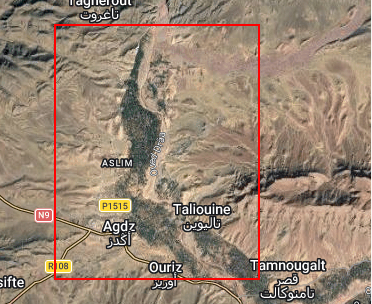
\includegraphics[
        width=0.88\textwidth,
        keepaspectratio
    ]{images/zone_etudier.png}

    \caption{Localisation de la zone d'étude d'Agdz dans la région Drâa-Tafilalet}
    \label{fig:zone_agdz}

\end{figure}

\vspace{0.4cm}
\renewcommand{\arraystretch}{1.35}
\begin{table}[H]
\centering
\renewcommand{\arraystretch}{1.4}

\begin{tabular}{|p{6cm}|p{8cm}|}
\hline
\rowcolor{blue!15}
\textbf{Paramètre} & \textbf{Description} \\
\hline

Localisation &
Province de Zagora, Région Drâa-Tafilalet, Maroc \\
\hline

Coordonnées &
30°41'N — 6°27'O \\
\hline

Altitude moyenne &
1169 m \\
\hline

Climat &
Semi-aride à tendance désertique \\
\hline

Température estivale &
Supérieure à 32°C durant la période estivale \\
\hline

Précipitations &
Faibles et irrégulières \\
\hline

Végétation &
Végétation clairsemée concentrée le long de l'Oued Drâa \\
\hline

\end{tabular}

\caption{Caractéristiques générales de la zone d'étude}
\label{tab:zone_etude}

\end{table}
\vspace{0.4cm}

\subsection{Sources de Données Mobilisées}

Le projet s'appuie sur trois catégories complémentaires de données environnementales, dont la combinaison constitue le socle analytique du système développé.

Les \textbf{images satellitaires Sentinel-2} de l'Agence Spatiale Européenne, accessibles via la plateforme Google Earth Engine, fournissent des données multispectrales à haute résolution (10 mètres) couvrant la zone d'étude. Ces images permettront de calculer les indices spectraux NDVI et NBR pour caractériser l'état du couvert végétal.

Les \textbf{données climatiques NASA POWER}, extraites via l'API publique de la NASA, couvrent la période 2017--2026 et renseignent les principales variables météorologiques de la région : température, humidité relative, précipitations et vitesse du vent. Ces séries temporelles constituent la base de l'analyse des conditions environnementales favorables aux incendies.

Les \textbf{données topographiques}, issues d'un modèle numérique de terrain (MNT), apportent les informations relatives au relief de la zone (altitude, pente, orientation des versants), variables complémentaires intégrées dans la modélisation du risque.

\subsection{Architecture Générale du Système}

Le système développé dans le cadre de ce projet s'organise autour d'une architecture intégrée en trois niveaux complémentaires.

Le premier niveau repose sur un \textbf{pipeline de collecte et de traitement des données} (ETL), qui automatise l'acquisition, le nettoyage et la structuration des données satellitaires et climatiques en vue de leur exploitation analytique.

Le second niveau correspond à la \textbf{modélisation prédictive} par l'algorithme Random Forest. Cet algorithme d'apprentissage supervisé a été retenu pour sa capacité à intégrer simultanément des variables de natures différentes — climatiques, spectrales et topographiques — et à produire une estimation spatialisée du niveau de risque d'incendie selon quatre classes : \textit{Faible}, \textit{Moyen}, \textit{Élevé} et \textit{Très élevé}.

Le troisième niveau est constitué d'un \textbf{tableau de bord interactif} développé sous le framework Streamlit. Cette interface centralisera la visualisation des données climatiques historiques, des résultats d'analyse des indices spectraux, des prédictions du modèle et de la cartographie du risque, offrant ainsi un outil de suivi dynamique et accessible aux gestionnaires du territoire.

% ============================================================
% CONCLUSION DU CHAPITRE 1
% ============================================================
\clearpage
\chapter*{Conclusion}
\addcontentsline{toc}{chapter}{Conclusion chapitre 2}

Ce premier chapitre a permis de poser les fondements contextuels et scientifiques du projet. La présentation de l'ORMVAO a mis en évidence le rôle stratégique de cet organisme dans le développement agricole et la gestion des ressources naturelles de la région de Drâa-Tafilalet, constituant ainsi un cadre institutionnel favorable à la conduite d'une étude environnementale appliquée.

La définition de la problématique a permis de cerner les enjeux spécifiques de la région d'Agdz, territoire semi-aride caractérisé par des conditions climatiques et végétales qui le rendent particulièrement vulnérable au risque d'incendie. Face à l'absence d'outils de surveillance adaptés, le recours aux technologies de télédétection, d'analyse géospatiale et d'apprentissage automatique s'impose comme une réponse pertinente et opérationnelle.

La méthodologie présentée, fondée sur l'intégration des images satellitaires Sentinel-2, des données climatiques NASA POWER et d'un modèle Random Forest, offre un cadre analytique cohérent et reproductible pour l'évaluation du risque d'incendie. L'architecture générale du système, articulée autour d'un pipeline de traitement, d'un module de modélisation prédictive et d'un tableau de bord interactif, constitue une base solide pour les développements qui seront détaillés dans les chapitres suivants.


% ============================================================
% CHAPITRE 2 — CONCEPTION DU SYSTÈME
% À intégrer dans le rapport principal après le Chapitre 1
% ============================================================

% ── PAGE DE TITRE DU CHAPITRE 2 ─────────────────────────────
\clearpage
\thispagestyle{empty}
\vspace*{\fill}
\begin{center}
  \rule{0.5\linewidth}{1.5pt}\\[1.2cm]
  {\fontsize{16}{20}\selectfont\bfseries\color{darkblue} CHAPITRE 2}\\[1cm]
  {\fontsize{18}{24}\selectfont\bfseries\color{darkblue}
    Conception du Système}\\[1.2cm]
  \rule{0.5\linewidth}{1.5pt}
\end{center}
\vspace*{\fill}
\clearpage

\chapter*{Chapitre 2 : Conception du Système}
\addtocontents{toc}{\protect\needspace{18\baselineskip}}
\addcontentsline{toc}{chapter}{Chapitre 2 \quad Conception du Système}
\setcounter{chapter}{2}
\setcounter{section}{0}
\setcounter{figure}{0}
\setcounter{table}{0}

% ── INTRODUCTION DU CHAPITRE ─────────────────────────────────
\section*{Introduction}
\addcontentsline{toc}{section}{Introduction}

La phase de conception constitue une étape déterminante dans le développement de tout système d'information, puisqu'elle assure la transition entre l'analyse des besoins et leur implémentation technique. Elle vise à structurer les données et à définir une architecture cohérente, capable de répondre aux exigences fonctionnelles et non fonctionnelles du projet.

Dans le cadre de ce travail, portant sur la conception d'un système de suivi et de prédiction des risques d'incendie dans la région d'Agdz, une approche méthodologique rigoureuse a été adoptée en s'appuyant sur la méthode \textbf{MERISE}. Cette dernière permet de modéliser le système à travers plusieurs niveaux d'abstraction complémentaires, garantissant ainsi une compréhension progressive et une implémentation maîtrisée.

Le \textbf{Modèle Conceptuel de Données (MCD)} permet de représenter les entités du domaine étudié ainsi que les relations qui les lient, indépendamment de toute contrainte technique. Le \textbf{Modèle Logique de Données (MLD)} traduit cette représentation en une structure relationnelle adaptée aux systèmes de gestion de bases de données. Enfin, le \textbf{Modèle Physique de Données (MPD)} concrétise cette modélisation à travers une implémentation en langage SQL, en intégrant les contraintes d'intégrité, les types de données appropriés ainsi que les mécanismes d'optimisation.

Par ailleurs, une attention particulière a été accordée à la qualité des données et au respect des règles de normalisation, afin d'assurer la cohérence, la fiabilité et la performance du système. L'intégration de données géospatiales, grâce à l'utilisation de \textbf{PostgreSQL} et de l'extension \textbf{PostGIS}, permet également d'enrichir l'analyse en tenant compte de la dimension spatiale, essentielle dans l'étude des phénomènes environnementaux tels que les incendies.

Ce chapitre présente ainsi l'ensemble des étapes de conception du système, depuis la modélisation conceptuelle jusqu'à l'implémentation physique, tout en mettant en évidence les choix techniques adoptés et les décisions d'architecture prises pour garantir un système robuste, évolutif et performant.

% ============================================================
% PARTIE 1 : MCD
% ============================================================
\section{Modèle Conceptuel des Données (MCD)}

\subsection{Objectif du MCD}

Le Modèle Conceptuel de Données (MCD) représente les données sous une forme abstraite, indépendante de toute technologie ou contrainte d'implémentation. Il décrit les \textbf{entités} (objets du monde réel pertinents pour le domaine étudié) et les \textbf{associations} (liens sémantiques entre entités), accompagnées de leurs cardinalités qui précisent le nombre d'occurrences possibles dans chaque relation.

Dans le contexte de ce projet, le MCD permet de formaliser les concepts fondamentaux liés à la surveillance du risque d'incendie : les zones géographiques, les données satellitaires, les indices de végétation, les variables climatiques, les périodes d'observation et les évaluations de risque. Cette modélisation constitue la fondation conceptuelle sur laquelle repose l'ensemble du système.

\begin{infobox}
La méthode MERISE (Méthode d'Étude et de Réalisation Informatique pour les Systèmes d'Entreprise) est une approche française de conception de systèmes d'information, structurée en niveaux d'abstraction successifs : conceptuel, logique et physique. Elle garantit une séparation claire entre la sémantique des données et leur implémentation technique.
\end{infobox}

\subsection{Liste des Entités Identifiées}

L'analyse du domaine a conduit à l'identification de six entités principales, chacune représentant un concept fondamental du système de surveillance des incendies :

\begin{table}[H]
\centering
\rowcolors{2}{lightgray}{white}
\begin{tabularx}{\textwidth}{L{3.5cm} L{4cm} X}
\toprule
\rowcolor{darkblue}
\textcolor{white}{\textbf{Entité}} &
\textcolor{white}{\textbf{Description}} &
\textcolor{white}{\textbf{Attributs principaux}} \\
\midrule
ZONE & Zone géographique étudiée &
  zone\_id, nom\_zone, superficie\_ha, latitude, altitude\_m, type\_vegetation, pente\_degre \\
IMAGE\_SATELLITE & Image acquise par satellite &
  image\_id, date\_acquisition, satellite \\
INDICE\_VEGETATION & Indice calculé (NDVI, NBR, dNBR) &
  indice\_id, type\_indice, valeur, date\_calcul, methode \\
DONNEE\_CLIMATIQUE & Données météorologiques &
  climat\_id, date\_mesure, temperature, precipitation, humidite \\
PERIODE & Intervalle de temps &
  periode\_id, date\_debut, date\_fin, saison \\
RISQUE\_INCENDIE & Résultat de l'analyse &
  risque\_id, niveau\_risque, score, date\_evaluation, methode\_calcul \\
\bottomrule
\end{tabularx}
\caption{Entités du Modèle Conceptuel de Données}
\label{tab:entites_mcd}
\end{table}

\subsection{Associations et Cardinalités}

Les associations entre entités traduisent les relations sémantiques du domaine. Chaque association est caractérisée par ses cardinalités minimale et maximale, qui précisent le nombre d'occurrences d'une entité pouvant participer à la relation.

\begin{table}[H]
\centering
\rowcolors{2}{lightgray}{white}
\begin{tabularx}{\textwidth}{L{2.8cm} L{4.5cm} C{2cm} X}
\toprule
\rowcolor{darkblue}
\textcolor{white}{\textbf{Association}} &
\textcolor{white}{\textbf{Entités}} &
\textcolor{white}{\textbf{Cardinalité}} &
\textcolor{white}{\textbf{Signification}} \\
\midrule
ACQUERIR & ZONE $\rightarrow$ IMAGE\_SATELLITE & 1,1 $\rightarrow$ 1,n &
  Une zone peut être couverte par plusieurs images satellitaires \\
EVALUER & ZONE $\rightarrow$ RISQUE\_INCENDIE & 1,1 $\rightarrow$ 1,n &
  Une zone peut faire l'objet de plusieurs évaluations de risque \\
MESURER & ZONE $\rightarrow$ DONNEE\_CLIMATIQUE & 1,1 $\rightarrow$ 1,n &
  Une zone dispose de plusieurs séries de mesures climatiques \\
CALCULER & IMAGE\_SATELLITE $\rightarrow$ INDICE\_VEGETATION & 1,1 $\rightarrow$ 1,n &
  Une image peut produire plusieurs indices spectraux \\
INFLUENCER & DONNEE\_CLIMATIQUE $\rightarrow$ RISQUE\_INCENDIE & 1,n $\rightarrow$ 1,1 &
  Les données climatiques influencent le niveau de risque \\
CONTRIBUER & INDICE\_VEGETATION $\rightarrow$ RISQUE\_INCENDIE & 1,n $\rightarrow$ 1,1 &
  Les indices de végétation contribuent à l'évaluation du risque \\
CONCERNER & PERIODE $\rightarrow$ RISQUE\_INCENDIE & 1,n $\rightarrow$ 1,1 &
  Une période peut être associée à plusieurs évaluations de risque \\
\bottomrule
\end{tabularx}
\caption{Associations et cardinalités du MCD}
\label{tab:associations_mcd}
\end{table}

\subsection{Schéma MCD Complet}

Le schéma MCD ci-dessous représente graphiquement l'ensemble des entités, de leurs attributs et des associations qui les relient. Les entités sont figurées par des rectangles, les associations par des ellipses, et les cardinalités sont indiquées sur chaque lien.

\begin{figure}[H]
    \centering
    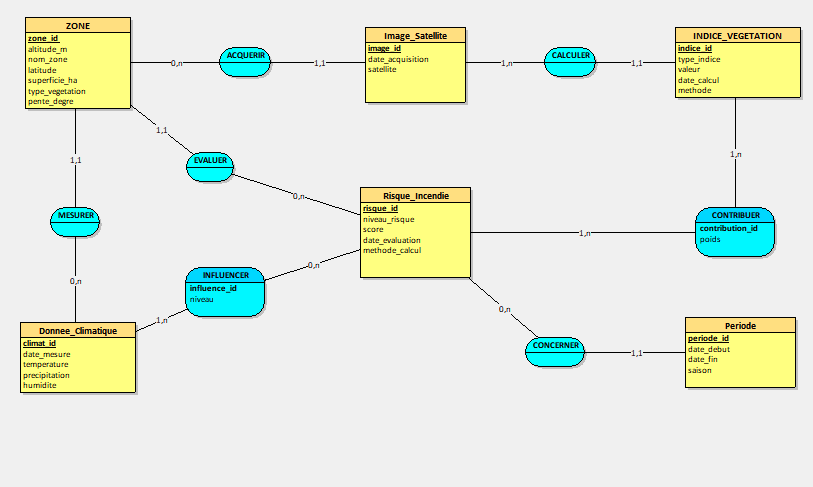
\includegraphics[width=0.92\textwidth]{images/mcd.png}
    \caption{Schéma du Modèle Conceptuel de Données (MCD)}
    \label{fig:mcd}
\end{figure}

\subsection{Dictionnaire des Données du MCD}

Le dictionnaire des données constitue la référence formelle de l'ensemble des attributs du modèle. Il précise, pour chaque entité, le type, la contrainte et la signification métier de chaque champ.

\begin{table}[H]
\centering
\rowcolors{2}{lightgray}{white}
\begin{tabularx}{\textwidth}{L{3.2cm} L{3cm} L{2.5cm} X}
\toprule
\rowcolor{darkblue}
\textcolor{white}{\textbf{Entité}} &
\textcolor{white}{\textbf{Attribut}} &
\textcolor{white}{\textbf{Type}} &
\textcolor{white}{\textbf{Description}} \\
\midrule
\multirow{7}{*}{ZONE}
  & zone\_id           & INTEGER     & Identifiant unique (PK) \\
  & nom\_zone          & VARCHAR(100)& Nom de la zone (ex : Agdz) \\
  & altitude\_m        & FLOAT       & Altitude en mètres \\
  & latitude           & FLOAT       & Latitude géographique (WGS84) \\
  & superficie\_ha     & FLOAT       & Superficie en hectares \\
  & type\_vegetation   & VARCHAR(50) & Type de végétation dominante \\
  & pente\_degre       & FLOAT       & Pente moyenne en degrés \\
\midrule
\multirow{3}{*}{IMAGE\_SATELLITE}
  & image\_id          & INTEGER     & Identifiant unique (PK) \\
  & date\_acquisition  & DATE        & Date de prise de vue \\
  & satellite          & VARCHAR(20) & Nom du satellite (ex : Sentinel-2) \\
\midrule
\multirow{5}{*}{INDICE\_VEGETATION}
  & indice\_id         & INTEGER     & Identifiant unique (PK) \\
  & type\_indice       & VARCHAR(10) & NDVI, NBR, dNBR, NDMI \\
  & valeur             & FLOAT       & Valeur calculée de l'indice \\
  & date\_calcul       & DATE        & Date du calcul \\
  & methode            & VARCHAR(50) & Méthode de calcul appliquée \\
\midrule
\multirow{4}{*}{DONNEE\_CLIMATIQUE}
  & climat\_id         & INTEGER     & Identifiant unique (PK) \\
  & date\_mesure       & DATE        & Date de la mesure \\
  & temperature        & FLOAT       & Température en °C \\
  & precipitation      & FLOAT       & Précipitations en mm \\
  & humidite           & FLOAT       & Humidité relative en \% \\
\midrule
\multirow{4}{*}{PERIODE}
  & periode\_id        & INTEGER     & Identifiant unique (PK) \\
  & date\_debut        & DATE        & Date de début de la période \\
  & date\_fin          & DATE        & Date de fin de la période \\
  & saison             & VARCHAR(20) & Saison (Printemps, Été, Automne, Hiver) \\
\midrule
\multirow{5}{*}{RISQUE\_INCENDIE}
  & risque\_id         & INTEGER     & Identifiant unique (PK) \\
  & niveau\_risque     & VARCHAR(20) & Faible, Moyen, Élevé, Très élevé \\
  & score              & FLOAT       & Score numérique (0--100) \\
  & date\_evaluation   & DATE        & Date de l'évaluation \\
  & methode\_calcul    & VARCHAR(50) & Méthode de classification utilisée \\
\bottomrule
\end{tabularx}
\caption{Dictionnaire des données du MCD}
\label{tab:dico_mcd}
\end{table}

% ============================================================
% PARTIE 2 : MLD
% ============================================================
\section{Modèle Logique des Données (MLD)}

\subsection{Règles de Transformation MCD $\rightarrow$ MLD}

Le passage du MCD au MLD obéit à des règles de transformation précises et systématiques. Chaque entité du MCD devient une table relationnelle, chaque attribut devient une colonne, et chaque identifiant devient une clé primaire. Les associations de cardinalité 1,n sont matérialisées par des clés étrangères dans la table du côté « n ». Les associations de cardinalité n,m donnent lieu à des tables de liaison autonomes.

\begin{table}[H]
\centering
\rowcolors{2}{lightgray}{white}
\begin{tabularx}{\textwidth}{L{5cm} X}
\toprule
\rowcolor{darkblue}
\textcolor{white}{\textbf{Règle de transformation}} &
\textcolor{white}{\textbf{Application dans ce projet}} \\
\midrule
Une entité devient une table &
  ZONE, IMAGE\_SATELLITE, DONNEE\_CLIMATIQUE, PERIODE, INDICE\_VEGETATION, RISQUE\_INCENDIE \\
Les attributs deviennent des colonnes &
  zone\_id, nom\_zone, altitude\_m, latitude\ldots \\
Les identifiants deviennent des clés primaires &
  \texttt{PRIMARY KEY (zone\_id)}, \texttt{PRIMARY KEY (image\_id)}\ldots \\
Les associations 1,n deviennent des clés étrangères &
  \texttt{FOREIGN KEY (zone\_id) REFERENCES ZONE} \\
Les associations n,m deviennent des tables de liaison &
  Tables INFLUENCER, CONTRIBUER, CONCERNER \\
\bottomrule
\end{tabularx}
\caption{Règles de transformation MCD vers MLD}
\label{tab:regles_mld}
\end{table}

\subsection{Schéma MLD}

\begin{figure}[H]
    \centering
    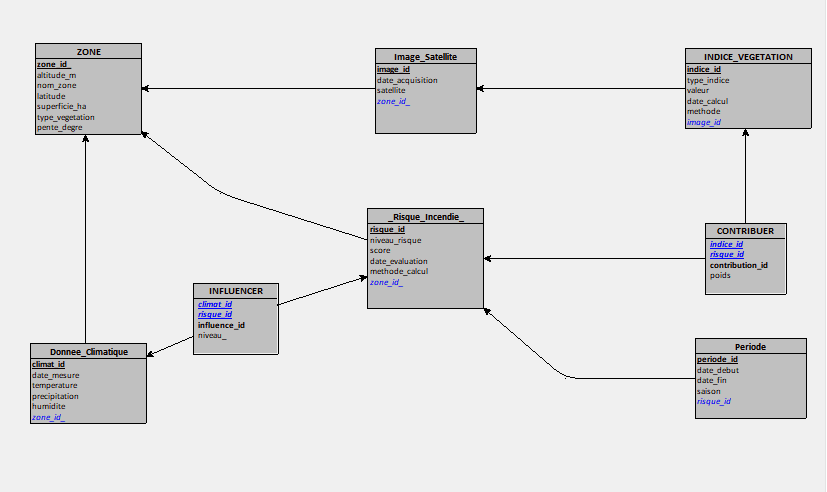
\includegraphics[width=0.92\textwidth]{images/mld.png}
    \caption{Schéma du Modèle Logique de Données (MLD)}
    \label{fig:mld}
\end{figure}

\subsection{Description des Tables du MLD}

Le modèle logique comprend neuf tables au total : six tables d'entités et trois tables d'association. La notation suivante est utilisée : les clés primaires sont soulignées, les clés étrangères sont précédées du symbole \#.

\vspace{0.3cm}
\begin{statusbox}
\textbf{ZONE} (\underline{zone\_id}, altitude\_m, nom\_zone, latitude, superficie\_ha, type\_vegetation, pente\_degre)
\quad PK : zone\_id

\vspace{0.4cm}
\textbf{IMAGE\_SATELLITE} (\underline{image\_id}, date\_acquisition, satellite, \#zone\_id)
\quad PK : image\_id \quad FK : zone\_id $\rightarrow$ ZONE(zone\_id)

\vspace{0.4cm}
\textbf{DONNEE\_CLIMATIQUE} (\underline{climat\_id}, date\_mesure, temperature, precipitation, humidite, \#zone\_id)
\quad PK : climat\_id \quad FK : zone\_id $\rightarrow$ ZONE(zone\_id)

\vspace{0.4cm}
\textbf{PERIODE} (\underline{periode\_id}, date\_debut, date\_fin, saison)
\quad PK : periode\_id

\vspace{0.4cm}
\textbf{INDICE\_VEGETATION} (\underline{indice\_id}, type\_indice, valeur, date\_calcul, methode, \#image\_id)
\quad PK : indice\_id \quad FK : image\_id $\rightarrow$ IMAGE\_SATELLITE(image\_id)

\vspace{0.4cm}
\textbf{RISQUE\_INCENDIE} (\underline{risque\_id}, niveau\_risque, score, date\_evaluation, methode\_calcul, \#zone\_id, \#periode\_id)
\quad PK : risque\_id \quad FK : zone\_id $\rightarrow$ ZONE(zone\_id) ; periode\_id $\rightarrow$ PERIODE(periode\_id)

\vspace{0.4cm}
\textbf{INFLUENCER} (\underline{influence\_id}, niveau, \#climat\_id, \#risque\_id)
\quad PK : influence\_id \quad FK : climat\_id $\rightarrow$ DONNEE\_CLIMATIQUE ; risque\_id $\rightarrow$ RISQUE\_INCENDIE

\vspace{0.4cm}
\textbf{CONTRIBUER} (\underline{contribution\_id}, poids, \#indice\_id, \#risque\_id)
\quad PK : contribution\_id \quad FK : indice\_id $\rightarrow$ INDICE\_VEGETATION ; risque\_id $\rightarrow$ RISQUE\_INCENDIE

\vspace{0.4cm}
\textbf{CONCERNER} (\underline{concerner\_id}, poids, \#risque\_id, \#periode\_id)
\quad PK : concerner\_id \quad FK : risque\_id $\rightarrow$ RISQUE\_INCENDIE ; periode\_id $\rightarrow$ PERIODE
\end{statusbox}

\subsection{Tableau Récapitulatif des Tables}

\begin{table}[H]
\centering
\rowcolors{2}{lightgray}{white}
\begin{tabularx}{\textwidth}{L{3.8cm} C{1.5cm} L{2cm} L{3cm} X}
\toprule
\rowcolor{darkblue}
\textcolor{white}{\textbf{Table}} &
\textcolor{white}{\textbf{Colonnes}} &
\textcolor{white}{\textbf{PK}} &
\textcolor{white}{\textbf{FK}} &
\textcolor{white}{\textbf{Types principaux}} \\
\midrule
ZONE              & 7 & zone\_id       & ---                    & INTEGER, VARCHAR, FLOAT \\
IMAGE\_SATELLITE  & 4 & image\_id      & zone\_id               & INTEGER, DATE, VARCHAR \\
DONNEE\_CLIMATIQUE & 6 & climat\_id    & zone\_id               & INTEGER, DATE, FLOAT \\
PERIODE           & 4 & periode\_id    & ---                    & INTEGER, DATE, VARCHAR \\
INDICE\_VEGETATION & 6 & indice\_id    & image\_id              & INTEGER, VARCHAR, FLOAT, DATE \\
RISQUE\_INCENDIE  & 6 & risque\_id     & zone\_id, periode\_id  & INTEGER, VARCHAR, FLOAT, DATE \\
INFLUENCER        & 4 & influence\_id  & climat\_id, risque\_id & INTEGER, VARCHAR \\
CONTRIBUER        & 4 & contribution\_id & indice\_id, risque\_id & INTEGER, FLOAT \\
CONCERNER         & 4 & concerner\_id  & risque\_id, periode\_id & INTEGER, FLOAT \\
\bottomrule
\end{tabularx}
\caption{Tableau récapitulatif des tables du MLD}
\label{tab:recap_mld}
\end{table}

% ============================================================
% PARTIE 3 : MPD
% ============================================================
\section{Modèle Physique des Données (MPD)}

\subsection{Principes de l'Implémentation Physique}

Le Modèle Physique de Données (MPD) constitue la concrétisation finale de la conception : il traduit le schéma logique en instructions SQL exécutables, adaptées au système de gestion de base de données cible. Dans ce projet, le SGBD retenu est \textbf{PostgreSQL} avec l'extension spatiale \textbf{PostGIS}, qui permet la gestion native des géométries et des requêtes spatiales.

Le script SQL intègre plusieurs mécanismes de qualité et d'optimisation :
\begin{itemize}
  \item des \textbf{contraintes d'intégrité} (\texttt{PRIMARY KEY}, \texttt{FOREIGN KEY}, \texttt{NOT NULL}) garantissant la cohérence référentielle ;
  \item des \textbf{contraintes de domaine} (\texttt{CHECK}) encadrant les valeurs acceptables ;
  \item la \textbf{suppression en cascade} (\texttt{ON DELETE CASCADE}) assurant la propagation des suppressions ;
  \item un \textbf{type géométrique} (\texttt{GEOMETRY(POLYGON, 4326)}) pour stocker les contours géospatiaux des zones.
\end{itemize}

\subsection{Script SQL Complet}

\subsubsection{Initialisation de la Base de Données}

\begin{verbatim}
-- ============================================
-- BASE DE DONNÉES : oasis_fires
-- ============================================
CREATE DATABASE oasis_fires;
\c oasis_fires;

-- Activation des extensions spatiales
CREATE EXTENSION IF NOT EXISTS postgis;
CREATE EXTENSION IF NOT EXISTS postgis_topology;
\end{verbatim}

\subsubsection{Table ZONE}

\begin{verbatim}
CREATE TABLE ZONE (
    zone_id       SERIAL PRIMARY KEY,
    altitude_m    FLOAT,
    nom_zone      VARCHAR(100) NOT NULL,
    latitude      FLOAT,
    superficie_ha FLOAT,
    type_vegetation VARCHAR(50),
    pente_degre   FLOAT,
    geometry      GEOMETRY(POLYGON, 4326)
);
\end{verbatim}

\subsubsection{Table IMAGE\_SATELLITE}

\begin{verbatim}
CREATE TABLE IMAGE_SATELLITE (
    image_id         SERIAL PRIMARY KEY,
    date_acquisition DATE NOT NULL,
    satellite        VARCHAR(20) DEFAULT 'Sentinel-2',
    zone_id          INTEGER NOT NULL,
    CONSTRAINT fk_image_zone
        FOREIGN KEY (zone_id) REFERENCES ZONE(zone_id)
        ON DELETE CASCADE
);
\end{verbatim}

\subsubsection{Table DONNEE\_CLIMATIQUE}

\begin{verbatim}
CREATE TABLE DONNEE_CLIMATIQUE (
    climat_id     SERIAL PRIMARY KEY,
    date_mesure   DATE NOT NULL,
    temperature   FLOAT,
    precipitation FLOAT,
    humidite      FLOAT,
    zone_id       INTEGER NOT NULL,
    CONSTRAINT fk_climat_zone
        FOREIGN KEY (zone_id) REFERENCES ZONE(zone_id)
        ON DELETE CASCADE,
    CONSTRAINT check_temperature
        CHECK (temperature BETWEEN -20 AND 60),
    CONSTRAINT check_humidite
        CHECK (humidite BETWEEN 0 AND 100),
    CONSTRAINT check_precipitation
        CHECK (precipitation >= 0)
);
\end{verbatim}

\subsubsection{Tables PERIODE, INDICE\_VEGETATION et RISQUE\_INCENDIE}

\begin{verbatim}
CREATE TABLE PERIODE (
    periode_id SERIAL PRIMARY KEY,
    date_debut DATE NOT NULL,
    date_fin   DATE NOT NULL,
    saison     VARCHAR(20),
    CONSTRAINT check_dates
        CHECK (date_debut <= date_fin),
    CONSTRAINT check_saison
        CHECK (saison IN ('Printemps','Été','Automne','Hiver'))
);

CREATE TABLE INDICE_VEGETATION (
    indice_id   SERIAL PRIMARY KEY,
    type_indice VARCHAR(10) NOT NULL,
    valeur      FLOAT,
    date_calcul DATE NOT NULL,
    methode     VARCHAR(50),
    image_id    INTEGER NOT NULL,
    CONSTRAINT fk_indice_image
        FOREIGN KEY (image_id)
        REFERENCES IMAGE_SATELLITE(image_id) ON DELETE CASCADE,
    CONSTRAINT check_type_indice
        CHECK (type_indice IN ('NDVI','NBR','dNBR','NDMI')),
    CONSTRAINT check_valeur_indice
        CHECK (valeur BETWEEN -1 AND 2)
);

CREATE TABLE RISQUE_INCENDIE (
    risque_id       SERIAL PRIMARY KEY,
    niveau_risque   VARCHAR(20) NOT NULL,
    score           FLOAT,
    date_evaluation DATE NOT NULL,
    methode_calcul  VARCHAR(50),
    zone_id         INTEGER NOT NULL,
    periode_id      INTEGER NOT NULL,
    CONSTRAINT fk_risque_zone
        FOREIGN KEY (zone_id) REFERENCES ZONE(zone_id)
        ON DELETE CASCADE,
    CONSTRAINT fk_risque_periode
        FOREIGN KEY (periode_id) REFERENCES PERIODE(periode_id)
        ON DELETE CASCADE,
    CONSTRAINT check_niveau_risque
        CHECK (niveau_risque IN
               ('Faible','Moyen','Élevé','Très élevé')),
    CONSTRAINT check_score
        CHECK (score BETWEEN 0 AND 100)
);
\end{verbatim}

\subsubsection{Tables d'Association}

\begin{verbatim}
CREATE TABLE INFLUENCER (
    influence_id SERIAL PRIMARY KEY,
    niveau       VARCHAR(20),
    climat_id    INTEGER NOT NULL,
    risque_id    INTEGER NOT NULL,
    CONSTRAINT fk_influencer_climat
        FOREIGN KEY (climat_id)
        REFERENCES DONNEE_CLIMATIQUE(climat_id)
        ON DELETE CASCADE,
    CONSTRAINT fk_influencer_risque
        FOREIGN KEY (risque_id)
        REFERENCES RISQUE_INCENDIE(risque_id)
        ON DELETE CASCADE
);

CREATE TABLE CONTRIBUER (
    contribution_id SERIAL PRIMARY KEY,
    poids           FLOAT,
    indice_id       INTEGER NOT NULL,
    risque_id       INTEGER NOT NULL,
    CONSTRAINT fk_contribuer_indice
        FOREIGN KEY (indice_id)
        REFERENCES INDICE_VEGETATION(indice_id)
        ON DELETE CASCADE,
    CONSTRAINT fk_contribuer_risque
        FOREIGN KEY (risque_id)
        REFERENCES RISQUE_INCENDIE(risque_id)
        ON DELETE CASCADE,
    CONSTRAINT check_poids CHECK (poids BETWEEN 0 AND 1)
);

CREATE TABLE CONCERNER (
    concerner_id SERIAL PRIMARY KEY,
    poids        FLOAT,
    risque_id    INTEGER NOT NULL,
    periode_id   INTEGER NOT NULL,
    CONSTRAINT fk_concerner_risque
        FOREIGN KEY (risque_id)
        REFERENCES RISQUE_INCENDIE(risque_id)
        ON DELETE CASCADE,
    CONSTRAINT fk_concerner_periode
        FOREIGN KEY (periode_id)
        REFERENCES PERIODE(periode_id)
        ON DELETE CASCADE
);
\end{verbatim}

\subsection{Indexation et Optimisation des Performances}

Au-delà des contraintes d'intégrité, des index ont été définis pour accélérer les requêtes les plus fréquentes. L'indexation porte notamment sur les clés étrangères (souvent utilisées dans les jointures) et les colonnes de type date (filtrages temporels).

\begin{verbatim}
-- Index sur les colonnes de recherche fréquente
CREATE INDEX idx_zone_nom
    ON ZONE(nom_zone);
CREATE INDEX idx_image_date
    ON IMAGE_SATELLITE(date_acquisition);
CREATE INDEX idx_climat_date
    ON DONNEE_CLIMATIQUE(date_mesure);
CREATE INDEX idx_indice_type
    ON INDICE_VEGETATION(type_indice);
CREATE INDEX idx_risque_niveau
    ON RISQUE_INCENDIE(niveau_risque);
CREATE INDEX idx_risque_date
    ON RISQUE_INCENDIE(date_evaluation);

-- Index spatial (PostGIS) sur la géométrie des zones
CREATE INDEX idx_zone_geometry
    ON ZONE USING GIST(geometry);
\end{verbatim}

\begin{table}[H]
\centering
\rowcolors{2}{lightgray}{white}
\begin{tabularx}{\textwidth}{L{4cm} L{3.5cm} X}
\toprule
\rowcolor{darkblue}
\textcolor{white}{\textbf{Index}} &
\textcolor{white}{\textbf{Table}} &
\textcolor{white}{\textbf{Justification}} \\
\midrule
idx\_zone\_nom         & ZONE                & Recherche rapide par nom de zone \\
idx\_image\_date       & IMAGE\_SATELLITE    & Filtrages temporels sur les acquisitions \\
idx\_climat\_date      & DONNEE\_CLIMATIQUE  & Sélection par période climatique \\
idx\_indice\_type      & INDICE\_VEGETATION  & Filtrage par type d'indice (NDVI, NBR\ldots) \\
idx\_risque\_niveau    & RISQUE\_INCENDIE    & Extraction des zones à risque élevé \\
idx\_risque\_date      & RISQUE\_INCENDIE    & Requêtes temporelles sur les évaluations \\
idx\_zone\_geometry    & ZONE (PostGIS)      & Requêtes spatiales optimisées (GIST) \\
\bottomrule
\end{tabularx}
\caption{Index définis pour l'optimisation des performances}
\label{tab:index}
\end{table}

\subsection{Normalisation (3NF)}

Le respect des formes normales garantit la cohérence des données et l'élimination de la redondance. Les trois premières formes normales ont été vérifiées pour l'ensemble des tables du modèle.

\begin{table}[H]
\centering
\rowcolors{2}{lightgray}{white}
\begin{tabularx}{\textwidth}{C{1.5cm} L{4.5cm} X}
\toprule
\rowcolor{darkblue}
\textcolor{white}{\textbf{Forme}} &
\textcolor{white}{\textbf{Description}} &
\textcolor{white}{\textbf{Vérification}} \\
\midrule
1NF & Pas de répétition de groupes &
  \checkmark{} Chaque colonne contient une valeur atomique et indivisible \\
2NF & Dépendance totale à la clé primaire &
  \checkmark{} Tous les attributs non-clés dépendent entièrement de la PK \\
3NF & Pas de dépendance transitive &
  \checkmark{} Aucun attribut non-clé ne dépend d'un autre attribut non-clé \\
\bottomrule
\end{tabularx}
\caption{Vérification de la normalisation (1NF, 2NF, 3NF)}
\label{tab:normalisation}
\end{table}

\subsection{Qualité des Données}

La qualité des données constitue un enjeu central pour la fiabilité des résultats du système. Cinq dimensions de qualité ont été définies et des mécanismes d'implémentation spécifiques ont été associés à chacune d'elles.

\begin{table}[H]
\centering
\rowcolors{2}{lightgray}{white}
\begin{tabularx}{\textwidth}{L{2.5cm} L{4cm} X}
\toprule
\rowcolor{darkblue}
\textcolor{white}{\textbf{Dimension}} &
\textcolor{white}{\textbf{Définition}} &
\textcolor{white}{\textbf{Implémentation}} \\
\midrule
Exactitude   & Données conformes à la réalité physique &
  Contraintes \texttt{CHECK} sur les valeurs numériques ; validation amont via GEE \\
Complétude   & Absence de valeurs manquantes critiques &
  \texttt{NOT NULL} sur toutes les colonnes essentielles (dates, identifiants, niveaux de risque) \\
Cohérence    & Absence de contradictions entre tables &
  \texttt{FOREIGN KEY} avec \texttt{ON DELETE CASCADE} ; contraintes inter-colonnes \\
Actualité    & Données à jour et représentatives &
  Vérification des dates d'acquisition ; couverture 2017--2026 \\
Unicité      & Absence de doublons &
  \texttt{PRIMARY KEY} sur chaque table ; \texttt{UNIQUE INDEX} sur les colonnes discriminantes \\
\bottomrule
\end{tabularx}
\caption{Les cinq dimensions de la qualité des données}
\label{tab:qualite}
\end{table}

% ============================================================
% PARTIE 4 : CHOIX TECHNIQUES
% ============================================================
\section{Choix Techniques et Architecture du Système}

\subsection{Choix du SGBD : PostgreSQL et PostGIS}

Le choix du Système de Gestion de Base de Données (SGBD) a été guidé par les exigences spécifiques du projet, notamment la nécessité de gérer des données spatiales (géométries polygonales des zones d'étude) et d'assurer une performance satisfaisante sur des volumes de données potentiellement importants (séries temporelles climatiques multi-annuelles, indices satellitaires).

\begin{table}[H]
\centering
\rowcolors{2}{lightgray}{white}
\begin{tabularx}{\textwidth}{L{3cm} C{3cm} C{3cm} C{3cm}}
\toprule
\rowcolor{darkblue}
\textcolor{white}{\textbf{Critère}} &
\textcolor{white}{\textbf{PostgreSQL}} &
\textcolor{white}{\textbf{MySQL}} &
\textcolor{white}{\textbf{Oracle}} \\
\midrule
Extension spatiale & PostGIS \checkmark{} & Faible support & Spatial (payant) \\
Open source        & Oui                  & Oui            & Non \\
Performance        & Très bonne           & Bonne          & Excellente \\
Coût               & Gratuit              & Gratuit        & Très élevé \\
Normalisation SQL  & Complète             & Partielle      & Complète \\
Support JSON/JSONB & Natif \checkmark{}   & Limité         & Partiel \\
Communauté         & Très active          & Active         & Commerciale \\
\bottomrule
\end{tabularx}
\caption{Comparaison des SGBD candidats}
\label{tab:sgbd}
\end{table}

PostgreSQL a été retenu pour son excellent support spatial via PostGIS, sa conformité aux standards SQL, son coût nul et la richesse de son écosystème. L'extension PostGIS ajoute les types \texttt{GEOMETRY} et \texttt{GEOGRAPHY}, ainsi que plus de 300 fonctions d'analyse spatiale (intersections, distances, projections, etc.), indispensables pour le traitement des données géographiques du projet.

\subsection{Types de Données Utilisés}

\begin{table}[H]
\centering
\rowcolors{2}{lightgray}{white}
\begin{tabularx}{\textwidth}{L{3.5cm} L{4cm} X}
\toprule
\rowcolor{darkblue}
\textcolor{white}{\textbf{Type SQL}} &
\textcolor{white}{\textbf{Utilisation}} &
\textcolor{white}{\textbf{Justification}} \\
\midrule
\texttt{SERIAL}              & Identifiants (zone\_id, etc.) &
  Auto-incrémentation automatique sans gestion applicative \\
\texttt{INTEGER}             & Compteurs, codes &
  Performances optimales pour les entiers sans décimale \\
\texttt{FLOAT}               & Mesures (température, superficie, valeurs d'indices) &
  Précision décimale suffisante pour les données environnementales \\
\texttt{VARCHAR(n)}          & Noms, descriptions, labels &
  Longueur contrôlée ; évite le gaspillage de stockage \\
\texttt{DATE}                & Dates d'acquisition, de mesure, d'évaluation &
  Opérations temporelles natives (intervalles, comparaisons) \\
\texttt{GEOMETRY(POLYGON, 4326)} & Contours géospatiaux des zones &
  PostGIS, système de référence WGS84 (standard GPS) \\
\bottomrule
\end{tabularx}
\caption{Types de données SQL utilisés dans le MPD}
\label{tab:types_sql}
\end{table}

\subsection{Architecture Globale du Pipeline de Données}

L'architecture du système de gestion des données s'articule autour d'un pipeline ETL (Extract, Transform, Load) structuré en trois phases distinctes et complémentaires :

\begin{enumerate}
  \item \textbf{Extraction (Extract)} : collecte automatisée des images Sentinel-2 via l'API Google Earth Engine et des données climatiques via l'API NASA POWER, en Python (bibliothèques \texttt{requests}, \texttt{earthengine-api}) ;
  \item \textbf{Transformation (Transform)} : nettoyage, normalisation et calcul des indices spectraux NDVI, NBR et dNBR ; jointures spatiales entre les données satellitaires et les zones d'étude dans QGIS et Python (\texttt{Pandas}, \texttt{GeoPandas}, \texttt{NumPy}) ;
  \item \textbf{Chargement (Load)} : insertion structurée des données traitées dans la base PostgreSQL/PostGIS via des scripts Python (\texttt{SQLAlchemy}, \texttt{psycopg2}), avec vérification des contraintes d'intégrité à chaque étape.
\end{enumerate}

\begin{figure}[H]
\centering
\begin{tabular}{c}
\fbox{\parbox{0.82\textwidth}{
\centering
\vspace{0.4cm}
{\small\textbf{SOURCES DE DONNÉES}}\\[0.2cm]
\textit{Google Earth Engine (Sentinel-2)} \quad | \quad \textit{NASA POWER API}\\[0.3cm]
$\downarrow$\\[0.2cm]
{\small\textbf{EXTRACTION (Python --- requests, earthengine-api)}}\\[0.3cm]
$\downarrow$\\[0.2cm]
{\small\textbf{TRANSFORMATION (Pandas, NumPy, GeoPandas, QGIS)}}\\
{\scriptsize Nettoyage --- Calcul NDVI/NBR --- Jointures spatiales --- Normalisation}\\[0.3cm]
$\downarrow$\\[0.2cm]
{\small\textbf{CHARGEMENT (SQLAlchemy --- PostgreSQL/PostGIS)}}\\[0.3cm]
$\downarrow$\\[0.2cm]
{\small\textbf{MODÉLISATION (Scikit-learn --- Random Forest)}}\\[0.3cm]
$\downarrow$\\[0.2cm]
{\small\textbf{VISUALISATION (Streamlit --- Folium --- QGIS)}}\\[0.4cm]
}}
\end{tabular}
\caption{Architecture globale du pipeline de données ETL}
\label{fig:pipeline}
\end{figure}

\subsection{Intégration des Composants du Système}

L'interopérabilité entre les différents composants du système constitue un facteur clé de sa robustesse. Le tableau suivant synthétise les interfaces et protocoles d'échange entre chaque brique technologique.

\begin{table}[H]
\centering
\rowcolors{2}{lightgray}{white}
\begin{tabularx}{\textwidth}{L{3cm} L{3.5cm} X}
\toprule
\rowcolor{darkblue}
\textcolor{white}{\textbf{Composant source}} &
\textcolor{white}{\textbf{Composant cible}} &
\textcolor{white}{\textbf{Interface / Format d'échange}} \\
\midrule
Google Earth Engine & Python (scripts ETL) & API REST ; GeoTIFF, GeoJSON \\
NASA POWER          & Python (scripts ETL) & API REST ; JSON \\
Python (ETL)        & PostgreSQL/PostGIS   & SQLAlchemy / psycopg2 ; SQL \\
PostgreSQL/PostGIS  & Python (ML)          & Pandas / SQLAlchemy ; DataFrame \\
Python (ML)         & Streamlit            & Objets Python natifs ; Pickle (modèle) \\
Streamlit           & Utilisateur final    & Interface web (navigateur) ; HTML/CSS/JS \\
QGIS                & Rapport / Dashboard  & PNG, SVG, GeoPackage \\
\bottomrule
\end{tabularx}
\caption{Interfaces d'intégration entre les composants du système}
\label{tab:integration}
\end{table}

% ============================================================
% CONCLUSION DU CHAPITRE 2
% ============================================================
\clearpage
\chapter*{Conclusion du Chapitre 2}
\addcontentsline{toc}{chapter}{Conclusion du Chapitre 2}

Au terme de ce chapitre, une modélisation complète et structurée du système de gestion et de prédiction des risques d'incendie dans la région d'Agdz a été établie. L'adoption de la méthode MERISE a permis de suivre une démarche progressive et rigoureuse, allant d'une représentation conceptuelle abstraite vers une implémentation physique concrète et optimisée.

Le \textbf{Modèle Conceptuel de Données (MCD)} a permis d'identifier et de structurer les six entités fondamentales du système --- ZONE, IMAGE\_SATELLITE, INDICE\_VEGETATION, DONNEE\_CLIMATIQUE, PERIODE et RISQUE\_INCENDIE --- ainsi que les sept associations qui les relient, avec leurs cardinalités précises. Cette modélisation garantit une représentation fidèle et exhaustive de la réalité du domaine environnemental étudié.

Le \textbf{Modèle Logique de Données (MLD)} a assuré la transformation de cette modélisation conceptuelle en un schéma relationnel cohérent, comprenant neuf tables au total, dont trois tables d'association matérialisant les relations de cardinalité complexe. La définition explicite des clés primaires et étrangères garantit l'intégrité référentielle de l'ensemble du modèle.

Le \textbf{Modèle Physique de Données (MPD)} a concrétisé cette conception à travers un script SQL intégrant des contraintes d'intégrité robustes, des types de données adaptés à chaque attribut et des mécanismes d'optimisation --- indexation classique et index spatial GIST --- visant à assurer la performance des requêtes, notamment les filtrages temporels et spatiaux.

Le respect des trois formes normales (1NF, 2NF, 3NF) a contribué à réduire la redondance et à garantir la cohérence des données, tandis que les cinq dimensions de qualité (exactitude, complétude, cohérence, actualité, unicité) ont été systématiquement prises en compte dans les choix d'implémentation. Le choix du SGBD PostgreSQL, couplé à l'extension PostGIS, s'est révélé particulièrement pertinent pour la gestion des données géospatiales, offrant des capacités avancées d'analyse géographique à coût nul.

Cette phase de conception constitue ainsi une base solide et évolutive pour le développement du système dans les chapitres suivants, notamment l'entraînement du modèle Random Forest et le déploiement du tableau de bord interactif Streamlit.
% ============================================================
\end{document}
